% This is LLNCS.DEM the demonstration file of
% the LaTeX macro package from Springer-Verlag
% for Lecture Notes in Computer Science,
% version 2.4 for LaTeX2e as of 16. April 2010
%
\documentclass{llncs}
\usepackage{graphicx}
%
\begin{document}
%
\title{Mobile Application Development with MELON}
%
\author{Justin Collins \and Rajive Bagrodia}
%
%%%% list of authors for the TOC (use if author list has to be modified)
\tocauthor{Justin Collins, Rajive Bagrodia}
%
\institute{University of California Los Angeles, Los Angeles CA, USA,\\
\email{\{collins, rajive\}@cs.ucla.edu}}

\maketitle

\begin{abstract}
Developing distributed applications for mobile ad hoc network continues to be challenging due to the dynamic and unpredictable nature of MANETs. MELON is a general purpose coordination language designed to provide flexible communication patterns for MANET applications while remaining lightweight. Based on a distributed shared message store, MELON abstracts network communication to an asynchronous exchange of persistent messages. MELON simplifies application development by supporting read-only and remove-only messages, bulk message retrieval, and per-host ordering of messages. In this paper, we review the MELON programming model, demonstrate its utility for writing MANET applications, and quantitatively compare it to traditional distributed computing paradigms in a MANET context.
\end{abstract}
%
\section{MELON Design}\label{sec:design}

The MELON communication paradigm borrows the idea of a distributed shared message store from Linda\cite{linda} and LIME\cite{lime}. The concept of tuple spaces - shared collections of messages which may be manipulated by many processes - fits well in a MANET context. To send a message, a process stores it in a globally shared memory "space". Messages are retrieved by matching them against desired templates. This decoupling between sending and receiving is beneficial in a MANET context, where maintaining connections between hosts can be challenging. With tuple spaces, disconnections no longer cause disruptions to communications, only delays in retrieving messages.

However, aside from the shared message store, MELON departs significantly from typical tuple spaces in its operations and semantics. In a tuple space, any message may be read or removed by any process, and any matching message may be retrieved in any order. For non-destructive reads, the same tuple may be returned multiple times. In contrast, MELON divides the messages into two pools: a remove-only pool, and a read-only pool. Remove-only messages can only be retrieved once and must be removed when retrieved. Read-only messages may never be explicitly removed, they can only be copied from the message store. Messages are returned in a per-host ordering, although which host returns a matching message remains nondeterministic.

Given the prevalence of private messages in current mobile applications (e.g., SMS, instant messaging, direct messaging in social applications), one further option for messages is to make them private. A take-only message may be given an addressee, which is the only process permitted to read the message.

MELON contains some additional minor differences from tuple spaces. First, messages are not required by the paradigm to be tuples, but may be implemented as any structure, given they can be matched by a template (for example, messages could be unordered tuples with named values instead). Secondly, considering the storage limitations of mobile devices, MELON explicitly limits the space available on a host for storing messages. As a result, messages may be automatically garbage collected. A last deviation from tuple spaces is the removal of strict semantics for returning messages. In tuple spaces, the semantics stipulate that if a matching message exists, it must be returned for a retrieval operation. In the reality of MANETs, this semantic cannot be met, so in MELON all retrieval operations are limited to best-effort.

These differences were introduced in MELON to both relieve the application developer of certain responsibilities and to allow the paradigm to operate well in a MANET. For example, read-only messages prevent a badly-behaved process from removing important messages meant to be read by many processes, and per-host ordering is especially convenient in applications such as news feeds or streaming video, where most messages are generated by a single host and the ordering is important. MELON is also deliberately designed to avoid any global state and allow for a completely distributed implementation.

\subsection{MELON Operations}

Processes in MELON communicate by storing messages to a distributed shared message store and retrieving the messages based on templates. In this paper, we assume messages consist of an ordered list of typed values. However, as noted above, nothing in the paradigm itself limits how messages might be constructed,  A message template is similar to a message, except it may contain both values and types. For example, a message containing \texttt{[1, "hello"]} could be matched by a template containing \texttt{[1, String]} or \texttt{[Integer, "hello"]} or \texttt{[Integer, String]}. A type will also match any subtypes.

Operations are split into read-only (\textbf{write}/\textbf{read}/\textbf{read\_all}) and take-only (\textbf{store}/\textbf{take}/\textbf{take\_all}) operations. Each operation is represented here as a separate function call. \textbf{store} and \textbf{write} operations have return null values and return as soon as the saved message is available in the message store (essentially immediately). \textbf{take} and \textbf{read} operations block by default until a matching message is returned, but may be set to non-blocking on a per-call basis. If a non-blocking call finds no matching messages, it returns an empty set.

\begin{table}
\centering
\begin{tabular}{|c|c|c|}
\hline
\textbf{Operation} & \textbf{Return Type} & \textbf{Action} \\ \hline
\textbf{store}(\textit{message}, \textit{[address]}) & \textit{null} & Store removable message \\ \hline
\textbf{write}(\textit{message}) & \textit{null} & Store read-only message \\ \hline
\textbf{take}(\textit{template}, \textit{[block = true]}) & \textit{message} or \textit{null} & Remove and return message \\ \hline
\textbf{read}(\textit{template}, \textit{[block = true]}) & \textit{message} or \textit{null} & Copy and return read-only message \\ \hline
\textbf{take\_all}(\textit{template}, \textit{[block = true]}) & \textit{array} & Bulk remove messages \\ \hline
\textbf{read\_all}(\textit{template}, \textit{[block = true]}) & \textit{array} & Bulk copy read-only messages \\ \hline
\end{tabular}
\caption{MELON Operations}
\end{table}

When called, \textbf{store} saves a copy of the message in the message store. Messages saved with \textbf{store} may only be retrieved with a \textbf{take} or \textbf{take\_all} operation. If an address is provided, then only the host with a matching identity can remove the message.

The \textbf{write} operation also stores a single message in the message store, but the message may only be copied from the storage space with a \textbf{read} operation, never explicitly removed. Messages written with the \textbf{write} operation may be automatically garbage collected.

A \textbf{take} operation requires a message template as the first argument and an optional boolean for the second argument. The message template is matched against available messages in the message store which were added with a \textbf{store} operation. If a matching message is found, it will be removed from the message store and returned. Once a message has been returned by a \textbf{take} operation, it may not be returned by a subsequent operation in any process.

The \textbf{read} operation will only return messages stored with a \textbf{write} operation which have not already been read by the current process. If a message matching the given message template is available, it will be copied and returned, but not removed from the message store. Once a message has been returned to a process, the message is considered to have been read by that process and will not be returned by any subsequent \textbf{read} or \textbf{read\_all} operations in that process. A message may be \textbf{read} by any number of processes, but only once per process.

\begin{table}
\centering
\caption{Read from multiple processes}
\begin{tabular}{|c|c|c|} \hline
\textbf{Process A} & \textbf{Process B} & \textbf{Process C} \\ \hline
\texttt{write([1, "hello"])} & \texttt{m = read([Integer, String])} & \texttt{m = read([Integer, String])} \\ \hline
\end{tabular}
\label{fig:readprocesses}
\end{table}

Table \ref{fig:readprocesses} illustrates one process writing a single message containing the integer \texttt{1} and the string \texttt{"hello"}. Processes B and C each perform a \textbf{read} operation with the template which matches the message stored by process A. Since \textbf{read} does not modify the storage space, the value of \textit{m} for both process B and C will be a copy of the message \texttt{[1, "hello"]} from process A.

The \textbf{take\_all} and \textbf{read\_all} operations are used to retrieve a group of matching messages instead of a single message. Otherwise, the semantics match \textbf{take} and \textbf{read}: \textbf{take\_all} can only remove messages from \textbf{store} operations, and \textbf{read\_all} only returns unread messages from \textbf{write} operations.

\begin{table}
\centering
\caption{News server and reader}
\begin{tabular}{|c|c|} \hline
\textbf{News Server} & \textbf{News Reader} \\ \hline
\begin{minipage}{2.45in}
\begin{verbatim}

function report(category, headline) {
   write([category, headline])
} 
\end{verbatim}
\end{minipage}
&
\begin{minipage}{2.5in}
\begin{verbatim}


function fetch(category) {
   return read_all([category, String])
}
\end{verbatim}
\end{minipage}
\\ \hline
\end{tabular}
\label{fig:newsreader}
\end{table}

Table \ref{fig:newsreader} demonstrates a use of \textbf{read\_all}. One or more processes generate news messages containing a news category and headline. To ensure all interested parties can read the news, the server uses \textbf{write} to disallow a reader from removing a news item and preventing other readers from reading it. Any number of processes can consume the news as readers. The \texttt{fetch} method in Table \ref{fig:readprocesses} uses \textbf{read\_all} to return all news items in a given category. Repeated calls to \texttt{fetch} will only return news items not previously seen.

By default, all retrieval operations will block the application until at least one matching message is found. The operations can also be performed in nonblocking mode, in which case \textbf{take} and \textbf{read} return null when no matching message is found, while \textbf{take\_all} and \textbf{read\_all} return empty collections.
   
\subsection{MELON Implementation}\label{sec:implementation}

\begin{figure}
\centering
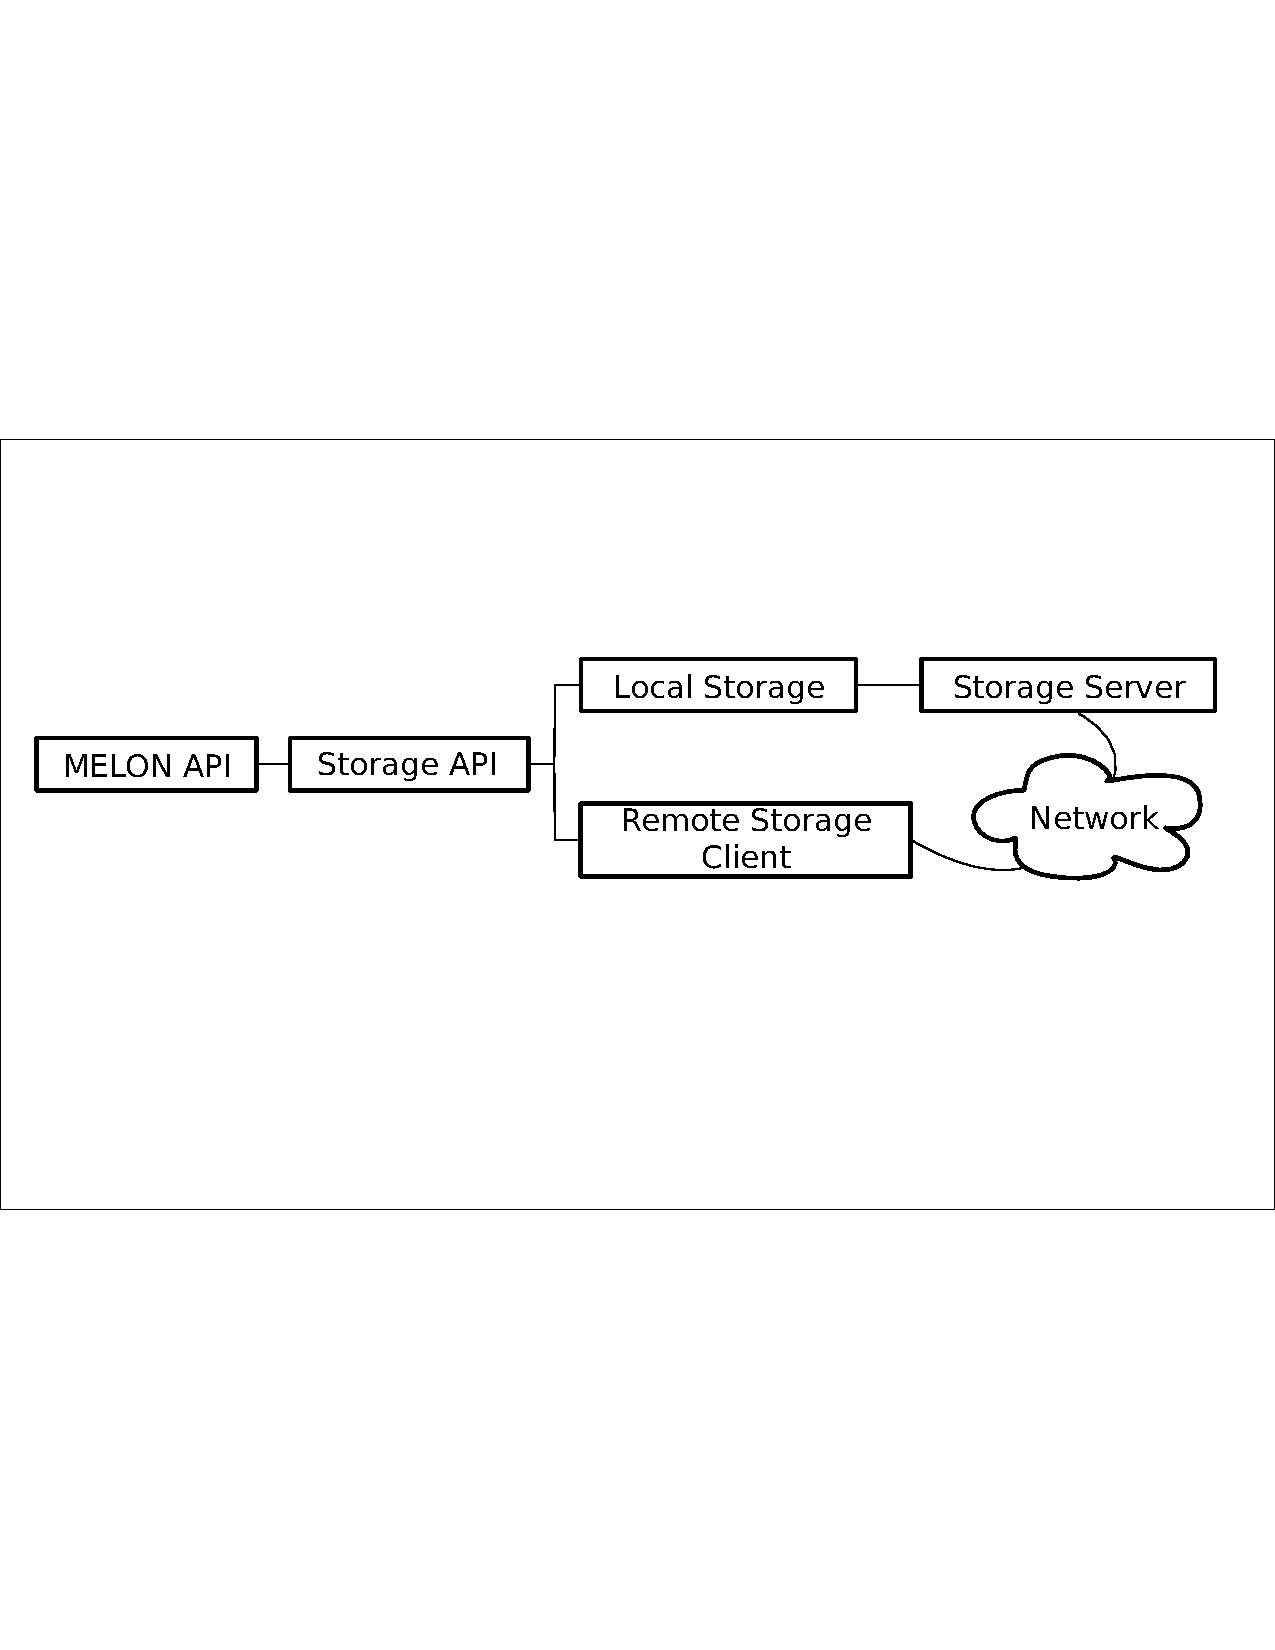
\includegraphics[scale = .50, clip, trim = 10px 350px 10px 312px]{figures/paradigm_arch.pdf}
\caption{Paradigm Architecture}
\label{fig:architecture}
\end{figure}

We developed a prototype implementation of MELON to validate our design and obtain empirical performance data. The architecture illustrated in Figure \ref{fig:architecture} is split into five parts. The MELON API is the only interface exposed to the application and provides the six operations described above. The MELON API interacts with the distributed message storage through the storage API, which provides the same interface for both local and remote storage. The storage server proves a network interface to a local storage space and accepts connections made through the remote storage stub.

Local storage is implemented as two dynamic arrays, one for \textbf{write}/\textbf{read} messages and the other for \textbf{store}/\textbf{take} messages. For atomic updates, the \textbf{write}/\textbf{read} array uses a readers/writer lock to allow multiple \textbf{read} operations to access the array concurrently, but locks the array for \textbf{write} operations. The \textbf{store}/\textbf{take} array does not permit concurrent operations, as \textbf{store} and \textbf{take} modify the store. The two arrays may be accessed and modified independently.

Network communication is handled using ZeroMQ\cite{hintjens2013zeromq}, a high performance networking library. For the prototype, the networking was intentionally kept simple. For example, a \textbf{read} request queries remote hosts in random order and stops when a matching result is returned. This could possibly be improved using multicast, but it would complicate the implementation by requiring the client to handle multiple asynchronous responses, select one, request the actual message, and handle failure scenarios if the matching message cannot be returned. We traded potential performance gains for simplicity. 

For \textbf{read} and \textbf{read\_all} operations, it is necessary to track which messages have been read. Each process maintains its own list of read messages, which it sends with each \textbf{read} request. We use a compact sparse bit set to track and transfer this information efficiently.

\section{Related Work}\label{sec:relatedwork}

The concept of a distributed shared message store is based on the idea of tuple spaces introduced with the Linda\cite{linda} coordination language. Several projects have adapted tuple spaces to MANETs, including LIME\cite{lime}, MESHmdl\cite{meshmdl}, TOTA\cite{tota}, and EgoSpaces\cite{egospaces}, of which LIME is likely the most well-cited example.

The original version of LIME relies on explicit join and leave operations to federate distributed tuple spaces, which is at odds with the frequently unexpected disconnections in MANETs. \cite{limerevisted} discusses the difficulties LIME encounters when attempting to implement tuple space semantics, including situations that can lead to livelocks. LIME II\cite{lime2}, Limone\cite{limone}, and CoreLIME\cite{corelime} are projects intended to address the shortcomings in the original LIME.

REDS\cite{reds} and GREEN\cite{green} are examples of publish/subscribe adapted to MANETS. AmbientTalk\cite{ambienttalk} is an entire language for MANETs based on RPC and actors. Further surveys of middleware, languages, and communication paradigms for MANET development can be found in \cite{mine} and \cite{mwtrends}.

\subsection{Comparison to Existing Paradigms}

This section compares MELON to publish/subscribe, remote procedure calls (RPC), and tuple spaces: three distributed computing paradigms often used as the basis for MANET middleware.

\subsubsection{Disconnection Handling}

In the unreliable MANET environment, disconnections frequently occur during the exchange of messages. Since disconnections can be prolonged, the networking layers will assume the connection is entirely lost and cease retrying. By having a message persist in some way, a paradigm can overcome these disconnections and deliver the message at a later time.

Publish/subscribe allows message publication without any consideration for the state of the subscribers. Publish/subscribe itself does not specify how ``missed'' publications should be handled. A publish/subscribe system can utilize ``brokers'' which manage subscriptions and facilitate delivery of publications. Brokers can then serve as message buffers and provide more reliable message delivery in the face of disconnections. In distributed publish/subscribe systems, however, the brokers must be self-organizing, and in MANET this is complicated by how quickly the network can change. It is common for distributed publish/subscribe systems not to provide message persistence. If a subscriber is not available at the time of publication, the message will not be received.

Since RPC requires a connection for communication, disconnections typically cause RPC to block a process entirely until a remote node hosting an appropriate method is available. Messages themselves only exist briefly during the RPC transaction. Messages cannot be sent if a connection cannot be made to a remote host.
    
In tuple spaces and MELON, message persistence is inherent in the paradigms. In both paradigms, exchange of messages is achieved by storing the messages in a shared storage space. Any amount of time may elapse between the storage of a message and its retrieval. This allows reliable communication even in the face of prolonged disconnections and is the reason we have chosen it for MELON.

\subsubsection{Addressing and Discovery}

All of the paradigms discussed here provide indirect addressing of resources separated from the physical machines. Publish/subscribe uses topics or content to deliver message to subscribers, RPC uses class and method names, and tuple spaces and MELON retrieve messages by matching content to templates. While all three traditional paradigms originally relied on centralized services (brokers from publish/subscribe, service directories for RPC, and a centralized database for tuple spaces), simple distributed versions may be implemented by having each node act as part of a distributed service.
    
\subsubsection{Flexible Communication}

A general purpose communication paradigm for MANET applications should have the flexibility to support both unicast and multicast communication.

Publications in publish/subscribe are inherently multicast, since any number of nodes can subscribe. Unicast communication is much less comfortable in publish/subscribe, as it involves negotiating which topics should be used to identify which nodes. Publish/subscribe also does not provide any mechanism for ensuring or even acknowledging message delivery to any given subscriber, especially since publishers and subscribers are intended to be unaware of each other.

Since RPC mimics local method calls, it is natural that RPC is best suited for unicast communication, in which the message is the argument to the method and the return value is the response from the remote host. Assuming multicast RPC functions in the same manner, then a multicast RPC invocation would expect multiple return values, one from each remote host. In a MANET, it is likely not every remote host would reliably return a response, further complicating the semantics. A typical RPC invocation would block waiting for a response, but it is not practical to wait for all responses to a multicast RPC invocation when some responses may never be received. The use of futures or asynchronous callbacks can improve the situation, but causes semantics to differ even more from unicast RPC.

Tuple spaces are naturally multicast, since any number of nodes may read a given tuple. Unicast communication can be achieved by using a field in the tuple as the recipient’s address. The recipient then performs in operations on tuples with their address in order to receive the tuples.

MELON divides communications into three types: messages which can be received by any single recipient, messages which can be received by a specific single recipient, and messages which can be received by any number of recipients. Messages sent with a store operation can only be consumed by a single take operation. Directed messages are also sent with store, but can only be consumed with a take performed by the intended recipient. write stores messages which may be read by any number of recipients and can never be removed by a take. MELON also provides the ability to receive multiple messages at once with \textbf{take\_all} and \textbf{read\_all} operations.
    
Networked applications also commonly require private, unicast communication. For example: SMS services, direct messaging in social networks, or communication of sensitive data. For our purposes, private communication is the exchange of messages between two parties which cannot be disrupted or eavesdropped upon by a third party from within the context of the paradigm itself. In other words, concerns such as encrypting data or sniffing network traffic would be outside the paradigm context.

RPC is unicast by default and there is no method in the paradigm for eavesdropping or disrupting RPC between two nodes. However, RPC has a different complication: remote hosts are generally identified by their exposed methods and there is no mechanism for attaching identity to the hosts. RPC will connect to any remote method with the expected API. So while private communication is the default in RPC, there is an addressing issue which makes it complicated to communicate with a specific recipient.

Communication in publish/subscribe is public and multicast by nature. Any subscriber can subscribe to any set of publications, making it simple to eavesdrop on communications. Bidirectional communication is also difficult in publish/subscribe, since there is no information attached to a publication indicating the identity of the publisher. This is by design, but it complicates situations in which two hosts need to dialog.

In tuple spaces, tuples are public and available to any recipient. Not only can any node read any communications without detection, any node can also disrupt communications by removing tuples intended for a specific recipient.

MELON provides two access control mechanisms for messages. First, messages are explicitly either available for any recipient to remove or limited to read-only operations. Read-only messages are useful in scenarios where information is intended to be widely available and removal of the information would be considered disruptive to the application. Second, if messages are directed to a specific recipient, then the paradigm implementation is responsible for disallowing any other nodes from reading or removing the given message. This allows simple private unicast communication between nodes.

\subsubsection{Multiple Read Problem}

The multiple read problem \cite{mrdp} is specific to tuple spaces: in a situation where the tuple space contains many tuples of interest, how do multiple readers read \textit{all} relevant tuples? In tuple spaces, the non-destructive \textbf{rd} operation returns a copy of a matching tuple, but it may return the same tuple any number of times since the tuple is chosen nondeterministically between all matching tuples. In many tuple space implementations, this occurs because the tuples are stored sequentially and so the first matching tuple is always the same\cite{de2012new}.

One solution is to use a single tuple as a mutex, lock the tuple space, remove all matching tuples with \textbf{in}, then replace them in the tuple space. However, this ruins any concurrency the tuple space could have had with multiple readers.

Another solution is to provide a bulk \textbf{rd} operation to return all matching tuples. However, once a ``snapshot'' of the tuple space has been taken with a bulk \textbf{rd}, new matching tuples may be introduced. A second bulk \textbf{rd} would return both the old (already seen) tuples and the new tuples. A similar suggestion from \cite{edwards2001jini} is to remove all matching tuples inside a transaction, then abort the transaction in order to actually leave the tuple space unmodified. However, this again leaves the problem of separating new tuples from previously-read tuples.

MELON avoids this issue by only returning messages unread by the current process. Assuming a fixed set of stored messages, repeated \textbf{read} operations in the same process would eventually return each matching message exactly once. MELON also provides the \textbf{read\_all} operation for reading messages in bulk. Unlike the tuple space version, \textbf{read\_all} only returns unread messages. This allows applications to easily read all existing matching messages, after which \textbf{read\_all} will only return messages stored since or unavailable during the previous operation.


\bibliographystyle{unsrt}
\bibliography{refs}

\end{document}
